\chapter{Results}
\label{sec:results}

This chapter will present results from the demonstrator to the reader.\\

%Things to evaluate: Overhead, memory usage, security stuff, economical benefit

%\section{Experiment design}
%Timer setup, etc

\section{Execution times}
This section covers the execution times of the tasks in the RTOS. Execution times were measured using a hardware timer on the FPGA with a resolution of 20 ns. All times were measured on the EMC\textsuperscript{2}DP. %The times were compared with oscilloscope measurements on an output pin where the pin was set high at the start of a task and set low at the end. This gave the same time as measured by the hardware timer, thus the hardware timer was deemed reliable.

\subsection{Data aggregation}
Data aggregation is the task with the highest frequency and priority in the system. It executes with a period of 1 ms. Data for its execution times can be seen in table~\ref{table:data_aggregation}.

\begin{table}[H]
\centering
\begin{tabular}{|l|c|c|}
\hline
 & Time & Clock cycles \\ \hline
WCET & 4 $\mu$s & 200 \\ \hline
BCET & 3.24 $\mu$s & 162 \\ \hline
Average ET & 3.38 $\mu$s & 169 \\ \hline
Median ET & 1.72 $\mu$s & 167 \\ \hline
Standard deviation & 0.1 $\mu$s & 5 \\ \hline
\end{tabular}
\caption{Execution times of data aggregation. Sample size: 6351}
\label{table:data_aggregation}
\end{table}

\subsection{Communication}
Communication is the task with the second highest priority. It executes with a period of 20 ms. Data for its execution times can be seen in table~\ref{table:communication}.

\begin{table}[H]
\centering
\begin{tabular}{|l|c|c|}
\hline
 & Time & Clock cycles \\ \hline
WCET & 6.32 $\mu$s & 316 \\ \hline
BCET & 3 $\mu$s & 150 \\ \hline
Average ET & 3.48 $\mu$s & 174 \\ \hline
Median ET & 3.02 $\mu$s & 151 \\ \hline
Standard deviation & 0.9 $\mu$s & 48 \\ \hline
\end{tabular}
\caption{Execution times of communication. Sample size: 3851}
\label{table:communication}
\end{table}

\subsection{Lateral control}
Lateral control is the task with the third highest priority, and executes with a period of 20 ms. It contains a timeout of 0.1 ms in a while loop as it waits for UART communication from the Raspberry Pi, which greatly affects its WCET. The execution times were measured when there was no communication via UART. Data for the tasks execution times can be seen in table~\ref{table:lateral_control}.%, since if the function always is timed out its execution time is very.

\begin{table}[H]
\centering
\begin{tabular}{|l|c|c|}
\hline
 & Time & Clock cycles \\ \hline
WCET & 104 $\mu$s & 5219 \\ \hline
BCET & 101 $\mu$s & 5061 \\ \hline
Average ET & 103 $\mu$s & 5155 \\ \hline
Median ET & 104 $\mu$s & 5200 \\ \hline
Standard deviation & 1.32 $\mu$s & 66 \\ \hline
\end{tabular}
\caption{Execution times of lateral control. Sample size: 878}
\label{table:lateral_control}
\end{table}

\subsection{Longitudinal control}
Longitudinal control is the task with the lowest priority in the RTOS. It executes with a period of 20 ms. Data for the tasks execution times can be seen in table~\ref{table:longitudinal_control}.

\begin{table}[H]
\centering
\begin{tabular}{|l|c|c|}
\hline
 & Time & Clock cycles \\ \hline
WCET & 4.6 $\mu$s & 230 \\ \hline
BCET & 3.62 $\mu$s & 181 \\ \hline
Average ET & 3.74 $\mu$s & 187 \\ \hline
Median ET & 3.7 $\mu$s & 185 \\ \hline
Standard deviation & 0.14 $\mu$s & 7 \\ \hline
\end{tabular}
\caption{Execution times of longitudinal control. Sample size: 4050}
\label{table:longitudinal_control}
\end{table}

\section{SafeG overhead}
To measure the overhead of SafeG monitor, a hardware timer was started on the secure side, immediately followed by a syscall to switch OS. The non-secure side immediately read the value of the timer and printed this value. This procedure was looped many times to gather a reliable set of data points. Pseudo code for this procedure follows below:\\

Secure side:
\begin{algorithmic}
\Loop
	\State $start\_timer()$
	\State $safeg\_syscall\_switch()$
\EndLoop
\end{algorithmic}

Non-secure side:
\begin{algorithmic}
\Loop
	\State $time\gets get\_time()$
	\State $reset\_timer()$
	\State $print(time)$
	\State $safeg\_syscall\_switch()$
\EndLoop
\end{algorithmic}

%According to TOPPERS~\cite{safegswitch}, this system switch should take at most 1.7 $\mu s$. 

This resulted in a data set of 103211 execution times, see table~\ref{table:switch_et}.

\begin{table}[H]
\centering
\begin{tabular}{|l|c|c|}
\hline
 & Time & Clock cycles \\ \hline
WCET & 3.06 $\mu$s & 153 \\ \hline
BCET & 0.96 $\mu$s & 48 \\ \hline
Average ET & 1.63 $\mu$s & 81 \\ \hline
Median ET & 1.72 $\mu$s & 86 \\ \hline
Standard deviation & 0.258 $\mu$s & 13 \\ \hline
\end{tabular}
\caption{Execution times of OS switch. Sample size: 103211}
\label{table:switch_et}
\end{table}

The measured execution times for the OS switch are also visualized in figure~\ref{fig:switch_et}.

\begin{figure}[H]
\centering
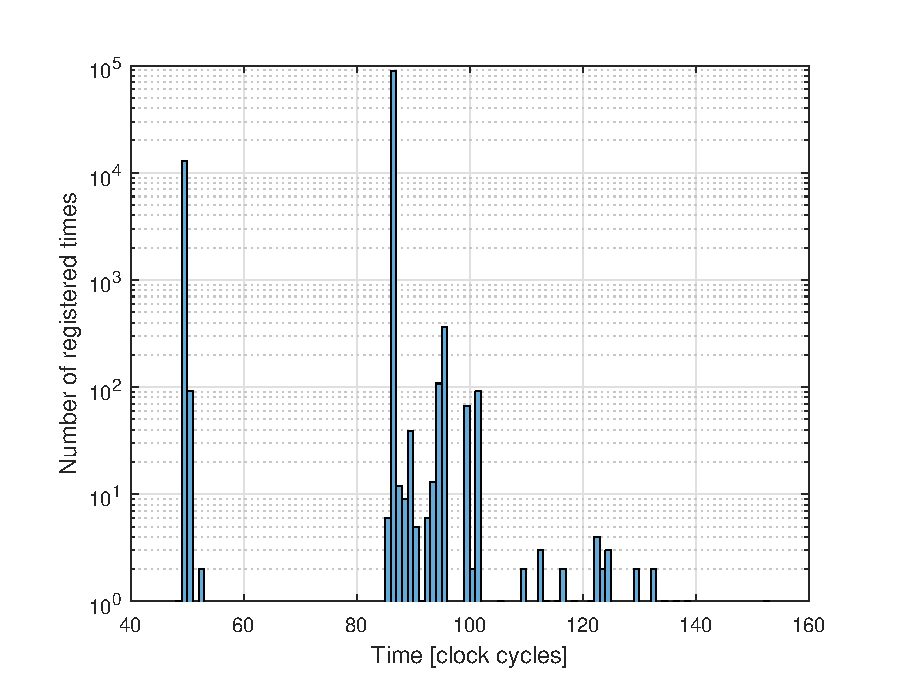
\includegraphics[width=\textwidth]{./img/results_switch_et.eps}
\caption{Visualization of execution times for the OS switch. Note the logarithmic y-axis.}\label{fig:switch_et}
\end{figure}

This results in an overhead of 0.6\% for the entire system. The potential useful CPU utilization is 99.4\%, providing that the GPOS uses all of its allocated CPU time. Using only the RTOS without the hypervisor the CPU utilization would be 0.005\%.\\

Theoretically, if FMP would allow for shorter periods for a task, the maximum overhead for this system would be 24\%.

\section{Hypervisor robustness}
To test the robustness of the hypervisor, a fork bomb was made on the GPOS. A fork bomb is a function that calls itself two times. This quickly depletes the system of its resources, causing it to crash eventually~\cite{forkbomb}. The test resulted in the GPOS crashing and becoming non-responsive while the RTOS managed to maintain all its functionality.\\

%Unregistered exception for a processor core was possible to create by accessing restricted AXI bus address, causing the processor to stop.\\
